%% Placeholder for chapter on convexity

%Below are notes for Oct23
\section{Linear/affine/convex/conic hulls \& sets}
Given a set of points $x^{(i)} \in \Re^n$, $i\in [m]$

\begin{equation*}
P = \{x^{(1)}, x^{(2)},..., x^{(m)} \}
\end{equation*}

Consider combinations of form $\sum^m_{i=1} \lambda_i x^{(1)}$

1) The "linear" hull: 

\begin{equation*}
\{x|x = \sum^m_{i=1} \lambda_i x^{(i)}, \lambda_r\in \Re, \forall i\in [m] \}
\end{equation*}

2) The "affine" hull: 

\begin{equation*}
\{x|x = \sum^m_{i=1} \lambda_i x^{(i)}, \lambda_i\in \Re, \sum^n_{i=1}\lambda_i = 1 \}
\end{equation*}


3) The "convex" hull: 

\begin{equation*}
\{x|x = \sum^m_{i=1} \lambda_i x^{(i)}, \lambda_i\in \Re, \lambda_i \geq 0, \sum^m_{i=1}\lambda_i = 1 \}
\end{equation*}


4) The "conic" hull: 

\begin{equation*}
\{x|x = \sum^m_{i=1} \lambda_i x^{(i)}, \lambda_i\in \Re, \lambda_i \geq 0 \}
\end{equation*}


\begin{center}
	\begin{tabular}{|c|c|c|}
	\hline  
   & $\lambda_i \geq 0$   & $\sum^m_{i=1}\lambda_i = 1$ \\
	\hline  
Linear&  no  & no \\
	\hline  
Affine&  no  &yes  \\
	\hline 
Covex&  yes  & yes \\
	\hline  
Conic&  yes  &  no\\
	\hline 
\end{tabular}
\end{center}



1) Linear Hull

Linear hull of $P = span\{x^{(1)},...,x^{(m)} \} =span(P)$

$\rightarrow$ smallest subspace that contains $P$.

2) Affine hull

\begin{align*}
P &= \{x^{(1)}, x^{(2)} \}\\
x &= \lambda_1x^{(1)} + \lambda_2x^{(2)}\\
&= \lambda_1x^{(1)} + (1-\lambda)_1x^{(1)}\\
&= x^{(2)} + \lambda(x^{(1)} - x^{(2)})\\
aff(P) &= x^{(2)} + span(x^{(1)} - x^{(2)})
\end{align*}

\begin{align*}
P &= \{x^{(1)}, x^{(2)}, x^{(3)} \}\\
x &= \lambda_1x^{(1)} + \lambda_2x^{(2)} + \lambda_3x^{(3)}\\
&= (1 - \lambda_2 - \lambda_3)x^{(1)} + \lambda_2x^{(2)} + \lambda_3x^{(3)}\\
&= x^{(1)} + \lambda_2(x^{(2)} - x^{(1)}) + \lambda_3(x^{(3)} - x^{(1)})
\end{align*}

\begin{marginfigure}
	\centering
	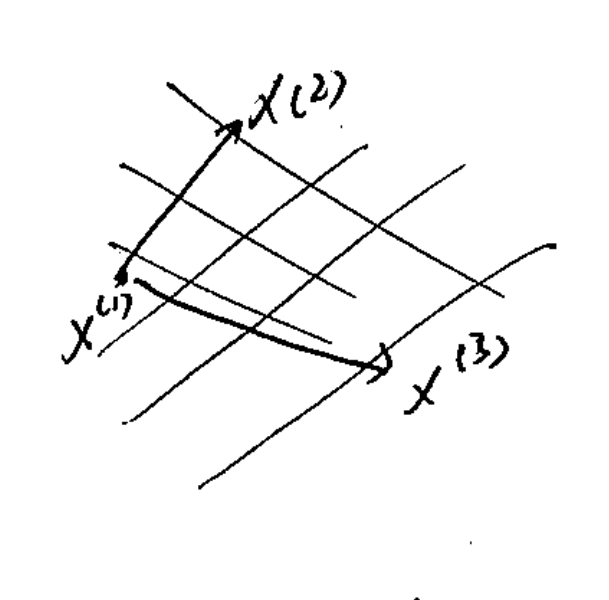
\includegraphics[width=1.8in,height=1.8in]{figures/ch07/figure1023_1.png}
	%\caption{This is an inserted JPG graphic} 
	%\label{fig:graph} 
\end{marginfigure}

3) Convex hulls

\begin{align*}
P &= \{x^{(1)},  x^{(2)}\}\\
x &= \lambda_1x^{(1)} + \lambda_2x^{(2)}\\
&= (1-\lambda)x^{(1)} + \lambda x^{(2)}\\
&= x^{(1)} + \lambda(x^{(2)} - x^{(1)})
\end{align*}

\begin{align*}
P &= \{x^{(1)},  x^{(2)}, x^{(3)} \}\\
x &= \lambda_1x^{(1)} + \lambda_2x^{(2)} + \lambda_3x^{(3)}\\
&= x^{(1)} + \lambda_2(x^{(2)} - x^{(1)}) + \lambda_3(x^{(3)} - x^{(1)})\\
&= x^{(1)} + \lambda \gamma(x^{(2)} - x^{(1)}) + (1 - \lambda)\gamma(x^{(3)} - x^{(1)})
\end{align*}


\begin{marginfigure}
	\centering
	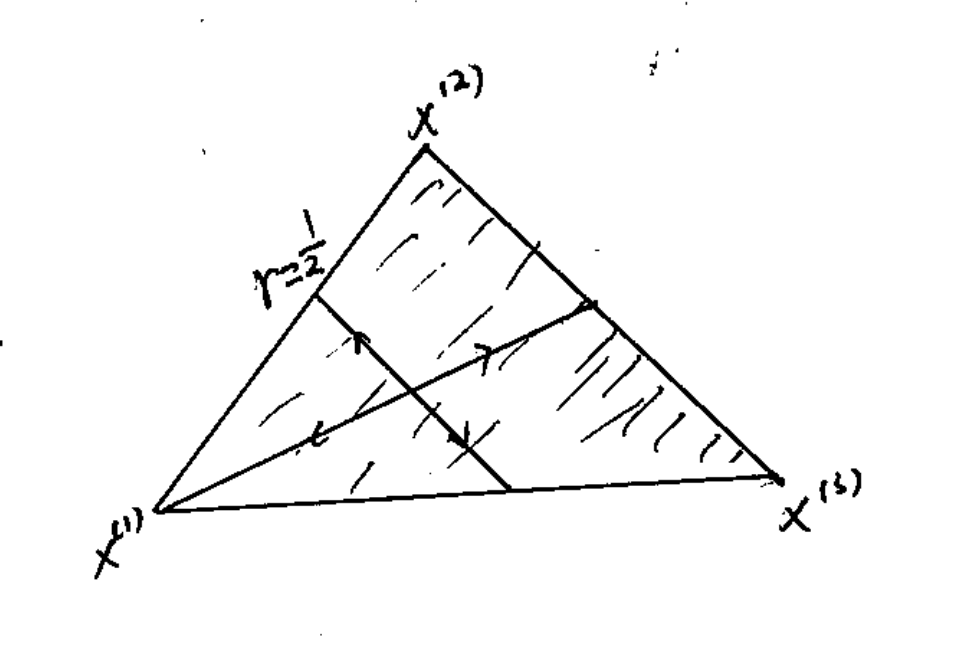
\includegraphics[width=1.8in,height=1.8in]{figures/ch07/figure1023_2.png}
	%\caption{This is an inserted JPG graphic} 
	%\label{fig:graph} 
\end{marginfigure}

\begin{marginfigure}
	\centering
	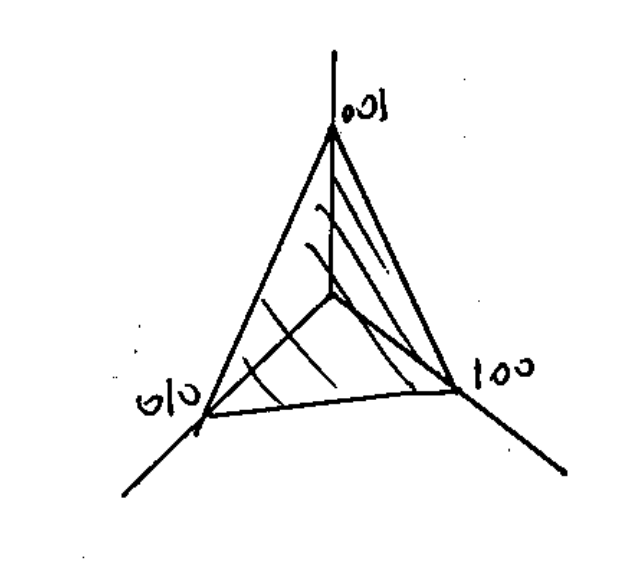
\includegraphics[width=1.8in,height=1.8in]{figures/ch07/figure1023_3.png}
	%\caption{This is an inserted JPG graphic} 
	%\label{fig:graph} 
\end{marginfigure}

4) Conic hulls: $\sum^n_{i=1}\lambda_i x^{(i)}$, $\lambda_i \geq 0$, $\forall i\in [m]$

\begin{align*}
P &= \{x^{(1)}, x^{(2)} \}\\
x &= \lambda_1x^{(1)} + \lambda_2x^{(2)}\\
&= ( \lambda_1 + \lambda_2)[\frac{\lambda_1}{\lambda_1 + \lambda_2}x^{(1)} + \frac{\lambda_2}{\lambda_1 + \lambda_2}x^{(2)}]\\
&= \gamma[\lambda x^{(1)} + (1-\lambda)x^{(2)}]
\end{align*}

\begin{marginfigure}
	\centering
	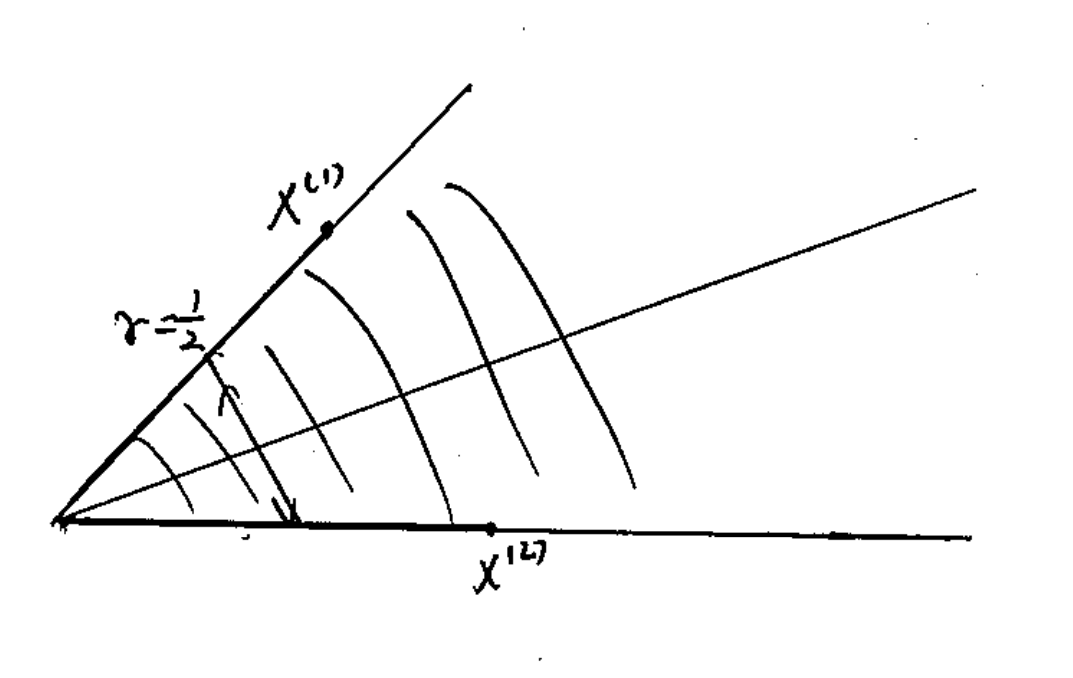
\includegraphics[width=1.8in,height=1.8in]{figures/ch07/figure1023_4.png}
	%\caption{This is an inserted JPG graphic} 
	%\label{fig:graph} 
\end{marginfigure}

\subsection{Convex Sets}

\begin{definition}{Convex}
	A subset $C\subseteq \Re^n$ is a "convex" set if $\forall x,y \in \mathcal{C}$, then $z\in \mathcal{C}$, $\forall z = \lambda x + (1-\lambda)y$, $\lambda \in [0,1]$
\end{definition}


\begin{definition}{Strictly Convex}
	A convex set is "strictly" convex if $\forall x,y \in \mathcal{C}$, $\forall \lambda \in (0,1)$, $z = \lambda x + (1-\lambda)y \in rel\,int(\mathcal{C})$(relative interior)
\end{definition}

Objects with straight edges are not strictly convex sets.

\begin{definition}{Cone}
	A set $\mathcal{C}\subseteq \Re^n $ is a cone if $\forall x\in \mathcal{C}$, then $\gamma x\in \mathcal{C}, \forall \gamma \geq 0$
\end{definition}

\begin{example}
	1) Hyper-planes are convex: $H = \{x| a^Tx = b \}$, pick $x,y \in H$, is $z =\lambda x + (1-\lambda)y \in H$? $\forall \lambda \in [0,1]$
	
	\begin{align*}
	a^Tz &= a^T(\lambda x + (1-\lambda)y)\\
	&= \lambda(a^Tx) + (1-\lambda)y\\
	&= \lambda b + (1-\lambda)b\\
	&= b
	\end{align*}
	
	
	2) Half-space: $\{x|a^Tx = b \}$, same proof except get inequality here in above equations($a^Tz \neq \lambda b + (1-\lambda)b$).
	
	3) If $c_1, ..., c_n$ al convex sets, then $\mathcal{C} = \cap^m_{i=1}$ is convex.
	
	\begin{proof}
		Pick any $x,y\in \mathcal{C}$ $\Rightarrow$ $x,y\in \mathcal{C}_i,\forall i\in [m]$.
		
		Consider any $z = \lambda x + (1 - \lambda)y$ , is this in $\mathcal{C}$?
		
		Since $x,y \in \mathcal{C}$, $\rightarrow z\in \mathcal{C}_i$ since $\mathcal{C}_i$, $\forall i\in [m]$
		
		If $z\in \mathcal{C}_i$, $\forall i\in [m]$ also intersection $\rightarrow z\in \cap^m_{i=1}C_i = C$
		
	\end{proof}

	In LP $\&$ QP Feasible set:
	
	\begin{equation*}
	\{x|Ax = b \}\cap \{x|Gx\leq b \} = \{\cap^q_{i=1}\{x|a^{(i)^T}x = b_i  \}\cap \{\cap^m_{i=1}\{x|g^{(i)^T}x \leq h_i \}
	\end{equation*}
	
	4) Affine transformations:
	
	If a map $F: \Re^n \rightarrow \Re^m$ is affine ($F(x) = Ax + b$) and $\mathcal{C} \subseteq \Re^n$ is convex, then the image of $\mathcal{C}$ under $F$ is convex.
	
	\begin{equation*}
	F(\mathcal{C}) = \{F(x) | x\in \mathcal{C} \} \subseteq \Re^m
	\end{equation*}

	Also pre-image of a convex set $\tilde{e}$ in $\Re^m$ is convex
	
	\begin{equation*}
	\{x|F(x)\in \mathcal{C} \} \subseteq \Re^n
	\end{equation*}
\end{example}

\begin{marginfigure}
	\centering
	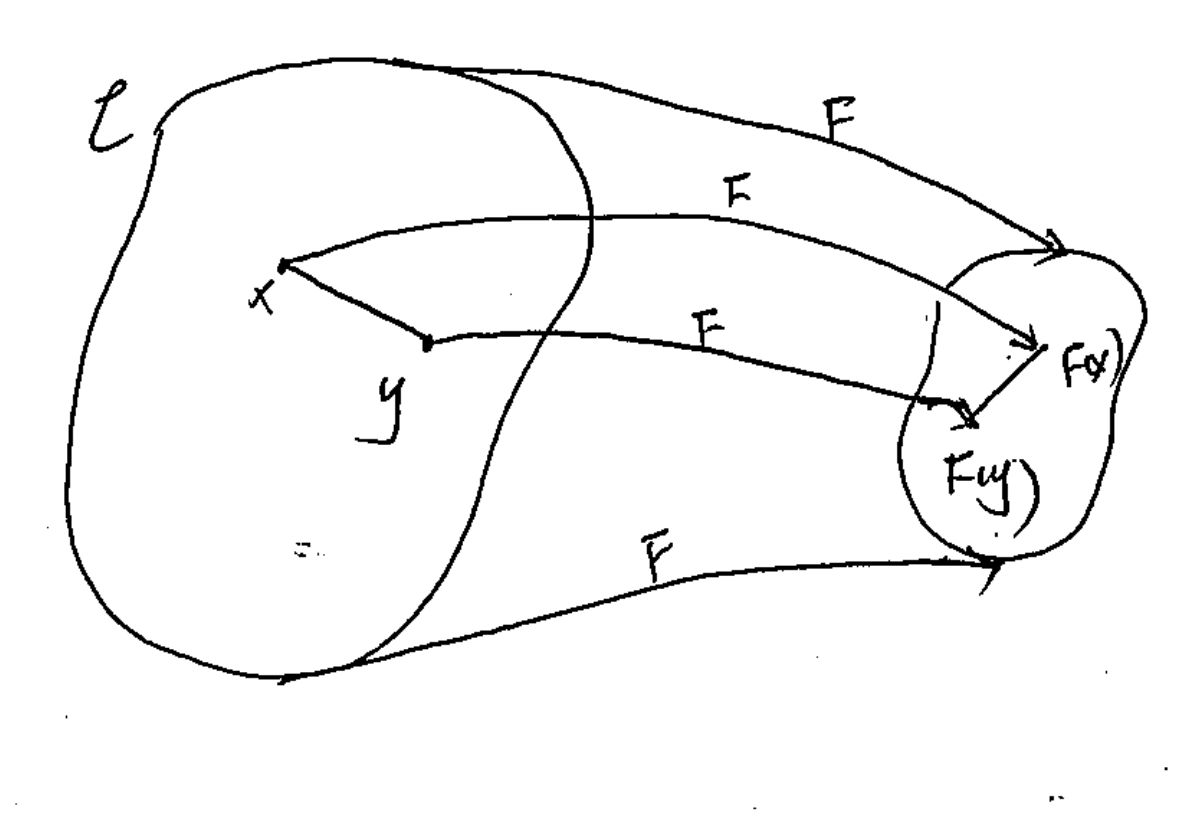
\includegraphics[width=1.8in,height=1.8in]{figures/ch07/figure1023_5.png}
	%\caption{This is an inserted JPG graphic} 
	%\label{fig:graph} 
\end{marginfigure}


Norm balls are convex

\begin{marginfigure}
	\centering
	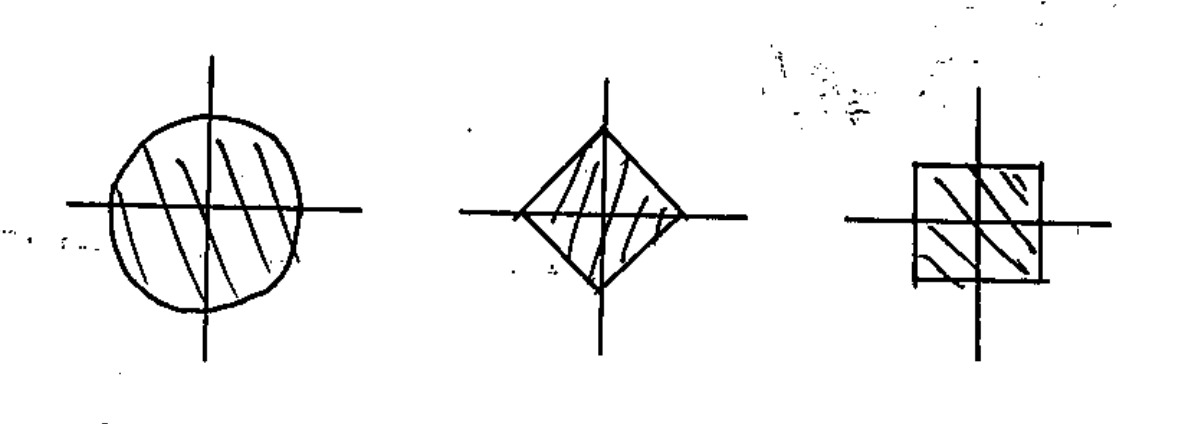
\includegraphics[width=1.8in,height=1.8in]{figures/ch07/figure1023_6.png}
	%\caption{This is an inserted JPG graphic} 
	%\label{fig:graph} 
\end{marginfigure}

\begin{proof}
	Take any two points $u,v$ s.t. $\Vert u\Vert \leq 1$, $\Vert v\Vert \leq 1$. 
	
	\begin{align*}
	\Vert \lambda u+(1-\lambda)v\Vert &\leq \Vert \lambda u\Vert + \Vert (1-\lambda)v\Vert\\
	&= \vert \lambda \vert \Vert  u\Vert + \vert (1-\lambda) \vert \Vert  v\Vert\\
	&= \lambda\Vert  u\Vert + (1-\lambda)\Vert  v\Vert\\
	&\leq \lambda 1 + (1-\lambda)1\\
	&= 1
	\end{align*}
	
	\begin{equation*}
	\Vert  x\Vert_p = (\sum^n_{i=1}\vert  x_i\vert^p)^{\frac{1}{p}}
	\end{equation*}
	norm if $p\geq 1$
\end{proof}

\subsection{Ellipsoids}

\begin{equation*}
\xi(x_c, P) =\{x|(x - x_c)^TP^{-1}(x - x_c) \leq 1 \}
\end{equation*}
where $P\in S^n_{++}$   is a convex set.

\begin{proof}
	
	$l_2$ norm ball is convex. 
	
	Consider following affine map $F(u) = P^{\frac{1}{2}}u + x_c$.
	
	The set $\{F(u) | \Vert y\Vert_2 \leq 1 \}$ is convex. 
\end{proof}

Define a set:

\begin{align*}
\{F(u) | \Vert u\Vert^2_2 \leq 1 \} &= \{x|x = P^{\frac{1}{2}}u+x_c, \Vert u\Vert^2 \leq 1 \}\\
&= \{x|x - x_c = P^{\frac{1}{2}}u, \Vert u\Vert^2 \leq 1 \}\\
&= \{x|P^{-\frac{1}{2}}(x - x_c) =u, \Vert u\Vert^2 \leq 1 \}\\
&= \{x|\Vert P^{-\frac{1}{2}}(x - x_c)\Vert^2_2 \leq 1 \}\\
&= \{x|(x - x_c)^TP^{-1}(x - x_c) \leq 1 \}
\end{align*}

Intersect these shapes with polyhedron to get feasible set of QCQP.

\begin{example}
	\begin{align*}
	\{x | \Vert Ax - b \Vert^2_2 \leq 1 \} &= \{x | \Vert F(x) \Vert^2 \leq 1 \}  where F(x) = Ax - b
	\end{align*}
	
	Pre-image of convex set under an affine function and so it's convex
\end{example}


%Above are notes for Oct23


%Below are notes for Oct30

%Above are notes for Oct30
